% !TEX root = ../patchEmbeddings_review.tex

\section{Related work} \label{sec:related_work}
\textbf{Proposal-based methods} -- Many of the recent successful instance segmentation methods on natural images are \emph{proposal based}: they first perform object detection, for example by predicting anchor boxes \cite{ren2015faster}, and then assign a class and a binary segmentation mask to each detected bounding box, either convolutionally \cite{he2017mask,porzi2019seamless,liu2018path,yang2012layered,li2017fully,ladicky2010and,hariharan2014simultaneous,chen2015multi,dai2016instance,liang2016reversible} or in a recurrent fashion by sequentially generating instances one-by-one \cite{romera2016recurrent,ren2017end}. 
However, in this work we focus on 3D neuron segmentation for connectomics, which is a field of neuroscience where instances/neurons cannot be approximated by bounding boxes. \TODO{Remove?}

\textbf{Proposal-free methods} on the other hand directly group pixels into instances. 
% whereas the template matching \cite{uhrig2016pixel} deploys scene depth information.
Recent approaches use metric learning to predict high-dimensional associative pixel embeddings that map pixels of the same instance close to each other, while mapping pixels belonging to different instances further apart, e.g. \cite{kong2018recurrentPix,fathi2017semantic,newell2017associative,de2017semantic} on natural images and \cite{lee2019learning} for neuron segmentation in connectomics. % kulikov2018instance
Final instances are then retrieved by applying a clustering algorithm and a post-processing step is needed to merge instances that are larger then the field of view of the network. 
Other proposal-free methods predict the relative coordinates of the instance center \cite{neven2019instance,cheng2019panopticdeeplab}, whereas others generate the mask of the instance associated to a given seed point \cite{sofiiuk2019adaptis} or  
learn a watershed transform by predicting its gradient direction \cite{bai2017deep}. 

\textbf{Aggregating \maskname masks} represents the line of research most related to ours. 
In \cite{liu2016multi}, densely located patches are predicted in a sliding window style across the entire image and the mask of an object is then generated by aggregating masks from overlapping patches.
In neuron segmentation, flood-filling networks \cite{januszewski2018high} and MaskExtend \cite{meirovitch2016multi} use a CNN to iteratively grow one region/neuron at the time; recently, the work of \cite{meirovitch2019cross} made the process more efficient by employing a combinatorial encoding of the segmentation.
The most closely related to ours is the unpublished work from \cite{hirsch2020patchperpix}, where... it has been applied to the BBBC010 benchmark microscopy dataset of \emph{C. elegans} worms.


\textbf{Patch aggregation}: \cite{liu2016multi} proposes to predict instance-aware masks in multi-scale patches and aggregate them to find all instances, sliding windows at a given stride on the image are used to generate these patches , related work suggested by Fred?



\begin{figure}[t]
\centering
        % \includegraphics[width=0.4\textwidth,trim=0.25in 0.25in 0.68in 0.36in,clip]{./figs/SSBM_experiments.pdf} % 0.45
        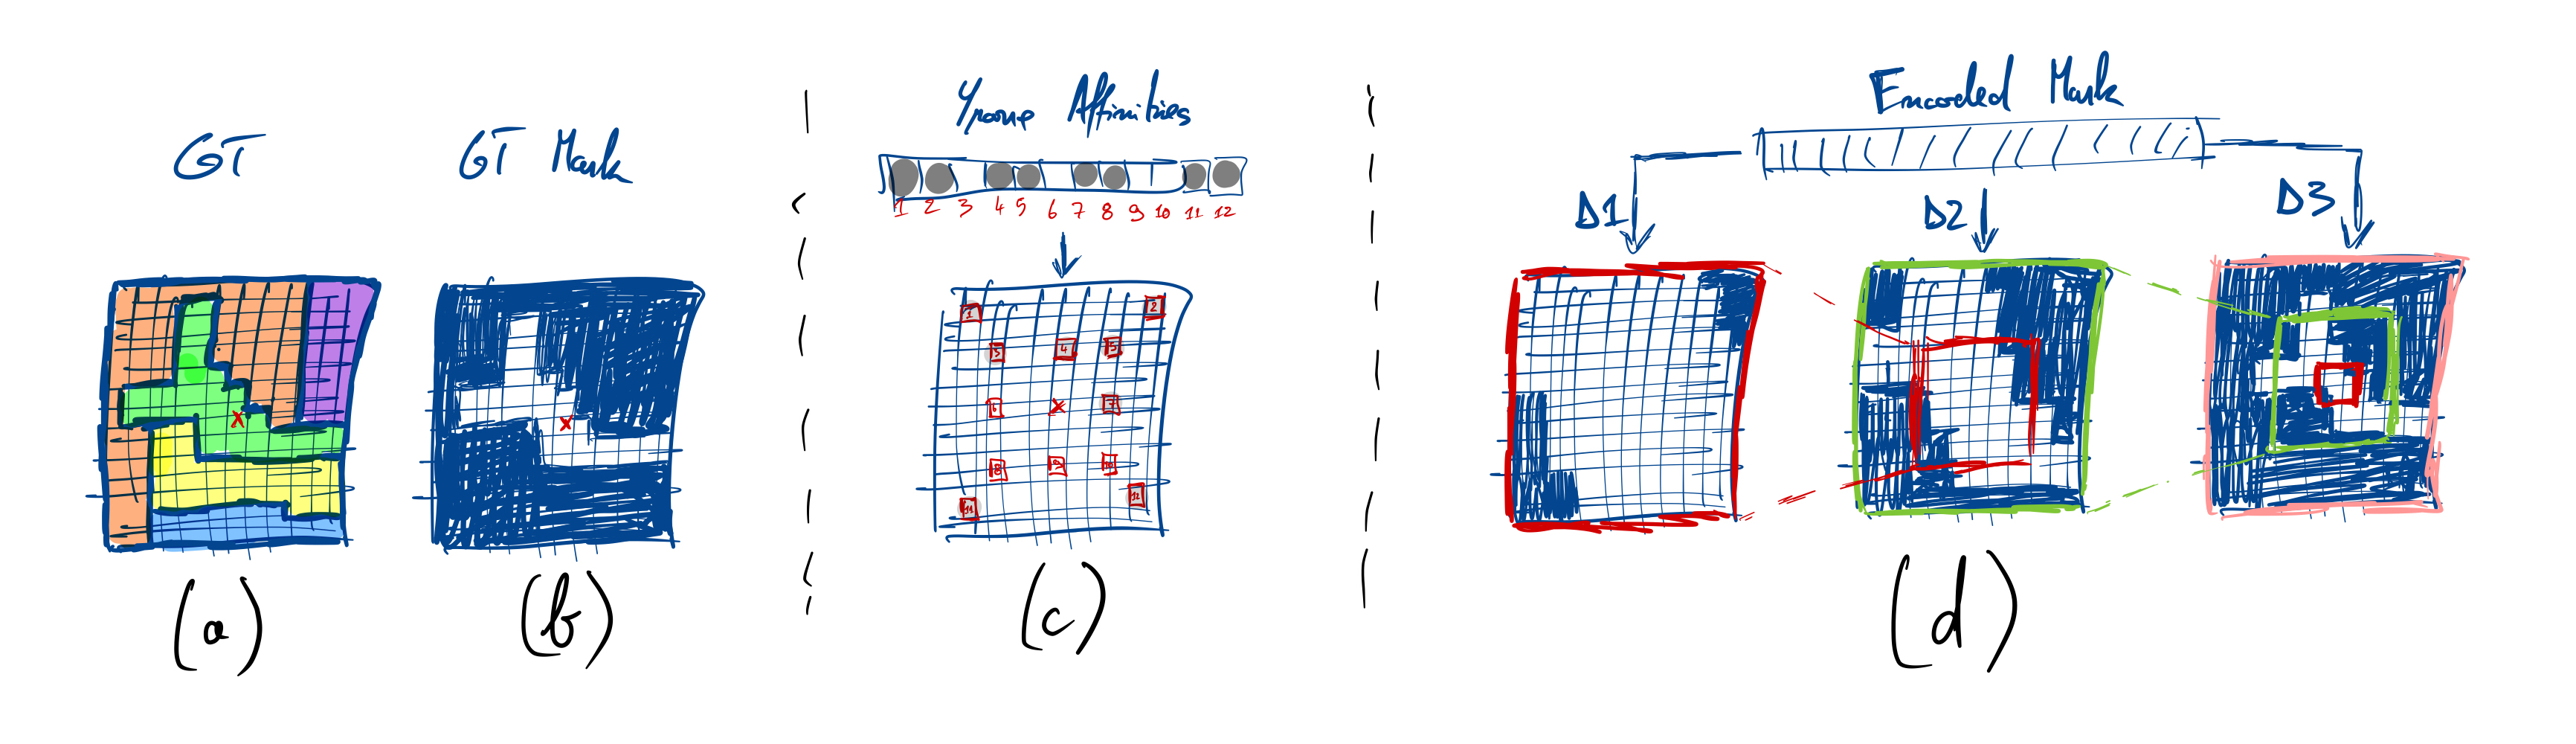
\includegraphics[width=\textwidth]{./figs/masks_explained.jpg} % 0.45
        \caption{Comparison between sparse affinities and encoded probability masks...}
    \label{fig:comparing_masks_affs}
\end{figure}





\textbf{Edge detection} 
For example, the approach proposed in \cite{kirillov2017instancecut} uses a combinatorial framework for instance segmentation

also experienced recent progress thanks to deep learning, both on natural images \cite{Gao_2019_ICCV,liu2018affinity,xie2015holistically,kokkinos2015pushing} and biological data \cite{lee2017superhuman,schmidt2018cell,meirovitch2016multi,ciresan2012deep}. In neuron segmentation for connectomics, a field of neuroscience we also address in our experiments, boundaries are converted to final instances with subsequent postprocessing and superpixel-merging:
some use loopy graphs \cite{kaynig2015large,krasowski2015improving} or trees \cite{meirovitch2016multi,liu2016sshmt,liu2014modular,funke2015learning,uzunbas2016efficient} to represent the region merging hierarchy; the lifted multicut \cite{beier2017multicut} formulates the problem in a combinatorial framework, whereas 

A structured learning approach was also proposed in \cite{funke2018large,turaga2009maximin}.

\TODO{}
 average linkage \cite{liu2018affinity,lee2017superhuman}, linkage learned by a random forest classifier \cite{nunez2013machine,knowles2016rhoananet}.


Extra approaches based signed graphs: Modern integer linear programming solvers can tackle problems of considerable size \cite{andres2012globally}, but accurate approximations \cite{pape2017solving,beier2016efficient,yarkony2012fast}, greedy agglomerative algorithms \cite{levinkov2017comparative,wolf2019mutex,keuper2015efficient,kardoostsolving} and persistence criteria \cite{lange2018partial,lange2018combinatorial} have been proposed for even larger graphs. 


proposal-free methods \cite{liu2018affinity,wolf2018mutex,lee2017superhuman} to predict long-range relationships between pixels.

\TODO{} patchPerPix, embeddings on connectomics, SSAP
% !!!!!!!!! TODO !!!!!!!!! : Related work from Fred


